\chapter{Two level system (Landau-Zener)}
\textit{\today\newline
Jan Střeleček\newline}

Let's have Hamiltonian
\begin{equation}
    \H(t)=\begin{pmatrix}
        \Omega(t)&\Delta(t)\\
        \Delta(t)&-\Omega(t)
    \end{pmatrix}
\end{equation}
and a driving along the path parametrized by time $t\in[0,1]$
\begin{equation}
    d(t)\coloneqq \begin{pmatrix}
        -s \cos(\omega(T_f)t)\\
        0\\
        s \sin(\omega(T_f)t)
    \end{pmatrix}
\end{equation}
for speed regulating function $\omega(T_f)\coloneqq \pi/T_f$. This means, the driving will always be along half-sphere, as in Fig. \ref{fig:driving}.

\begin{figure}[H]
    \centering
    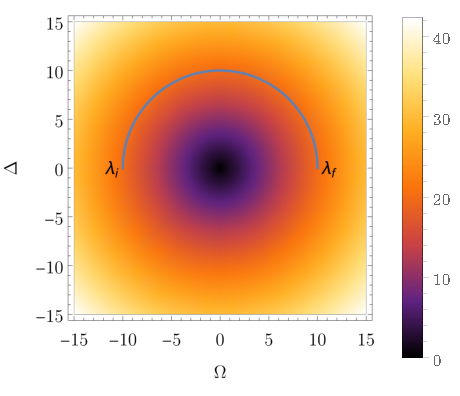
\includegraphics[scale=1.2]{../img/driving.pdf}
    \caption{Driving along the geodesic. $\lambda_i$ and $\lambda_f$ are initial resp. final parameters. DensityPlot shows the difference between Hamiltonian eigenvalues.}
    \label{fig:driving}
\end{figure}

\section{Derivation of the fidelity}
Because the Hamiltonian can be rewritten using Pauli matrices
\begin{equation}
    \H(t) = 
        \begin{pmatrix}
         -s \cos (t \omega ) & s \sin (t \omega ) \\
         s \sin (t \omega ) & s \cos (t \omega ) \\
        \end{pmatrix}
        =\Delta(t)\sigma_x+ \Omega(t)\sigma_z= d(t).\mathbf{\hat\sigma}
\end{equation}
one can see that changing from the \textcolor{purple}{original frame} to \textcolor{blue}{moving frame of reference} (let's omit the final time dependence $\omega=\omega(T_f)$ for a while) 
\begin{equation}
    \textcolor{purple}{\psi(t)} \eqqcolon \expsp \textcolor{blue}{\tilde\psi(t)}
\end{equation}
reflects rotational symmetry of the problem. This change of reference frame transforms Schr\"odinger equation
\begin{equation}
    \begin{split}
        \textcolor{purple}{\H(t)\psi(t)} &= i\textcolor{purple}{\psi'(t)}\\
        \textcolor{purple}{\H(t)} \expsp\textcolor{blue}{\tilde\psi(t)} &= i \expsp \left(\frac{i\omega\hat\sigma_y}{2}\right)\textcolor{blue}{\tilde\psi(t)}+i\expsp\textcolor{blue}{\tilde\psi'(t)}\\
        \underbrace{\left(\expsm \textcolor{purple}{\H(t)}\expsp+ \frac{\omega}{2}\hat\sigma_y\right)}_{\textcolor{blue}{\tilde\H(t)}}\textcolor{blue}{\tilde\psi(t)}&=i\textcolor{blue}{\tilde\psi'(t)}.
    \end{split}
\end{equation}
Therefore we can equivalently solve the Fidelity problem in this new coordinate system.

Hamiltonian in the moving frame is
\begin{equation}
    \textcolor{blue}{\tilde\H}=\textcolor{blue}{\begin{pmatrix}
        -s&-i\omega(T_f)/2\\
        i\omega(T_f)/2&s
    \end{pmatrix}},
\end{equation}
which is time independent. The Schr\"odinger equation can now be easily solved using evolution operator
\begin{equation}
    \begin{split}
        \textcolor{blue}{\UU(t)}=&e^{-i\textcolor{blue}{\tilde\H}t}\\
        =&\textcolor{blue}{\begin{pmatrix}
            \cos \left(\frac{t}{2} q(T_f)\right)+\frac{2 i s \sin \left(\frac{t}{2} q(T_f)\right)}{q(T_f)} & -\frac{\omega(T_f)  \sin \left(\frac{t}{2} q(T_f)\right)}{q(T_f)} \\
            \frac{\omega(T_f)  \sin \left(\frac{t}{2} q(T_f)\right)}{q(T_f)} & \cos \left(\frac{t}{2} q(T_f)\right)-\frac{2 i s \sin \left(\frac{t}{2} q(T_f)\right)}{q(T_f)} \\
        \end{pmatrix}},
    \end{split}
\end{equation}
for $q(T_f)=\sqrt{4 s^2+\omega(T_f) ^2}$.

In the original frame we get the evolution of the state $\psi(0)$
\begin{equation}
    \textcolor{purple}{\psi(t)}=\expsp \textcolor{blue}{\UU(t) \tilde\psi(0)} = \underbrace{\expsp \textcolor{blue}{\UU}\expsm}_{\textcolor{purple}{\UU(t)}} \underbrace{\expsp \textcolor{blue}{\tilde\psi(0)}}_{\textcolor{purple}{\psi(0)}}.
\end{equation}
Then the evolved wavefunction is
\begin{equation}
    \textcolor{purple}{\ket{\psi(t)}}=\textcolor{purple}{\begin{pmatrix}
        \cos \left(\frac{t}{2} q(T_f)\right)+\frac{2 i s \cos (t \omega(T_f) ) \sin \left(\frac{t}{2} q(T_f)\right)}{q(T_f)}\\
        \frac{(\omega(T_f) -2 i s \sin (t \omega(T_f) )) \sin \left(\frac{t}{2} q(T_f)\right)}{q(T_f)}
    \end{pmatrix}}
\end{equation}
and the ground state
\begin{equation}
    \textcolor{purple}{\ket{0(t)}}=\textcolor{purple}{\mathcal{N}\begin{pmatrix}
        -\cot (\frac{t}{2}\omega(T_f))\\
        1
    \end{pmatrix}},
\end{equation}
for a normalization constant $\textcolor{purple}{\mathcal{N}}\coloneqq |\textcolor{purple}{\braket{0(t)|0(t)}}|^{-1}$.
Fidelity during the transport is then\footnote{If we would calculate the Fidelity in \textcolor{blue}{comoving frame}, we would get exactly one. This is the essence of counterdiabatic driving.}
\begin{equation}
    F=\left|\textcolor{purple}{\braket{0(t)|\psi(t)}}\right|^2,
\end{equation}

 Explicit formula for fidelity in time $t$ and geodesic driving with final time $T_f$ is then
\begin{equation}
    F(t,T_f)=\frac{\pi ^2 \left(\cos \left(t \sqrt{\frac{\pi ^2}{T_f^2}+4 s^2}\right)+1\right)+8 s^2 T_f^2}{2 \sin ^4\left(\frac{\pi  t}{2 T_f}\right) \left(4 s^2 T_f^2+\pi ^2\right) \left(\left| \cot \left(\frac{\pi  t}{2 T_f}\right)\right|^2+1\right)^2}.
    \label{eq:fidelitySimplified}
\end{equation}


\section{Analysis of the fidelity formula}
Fidelity for some fixed final time is just oscilating curve close to $1$. For $T_f=10$ it can be seen on Fig. \ref{fig:infidelityTimePlot}
\begin{figure}[H]
    \centering
    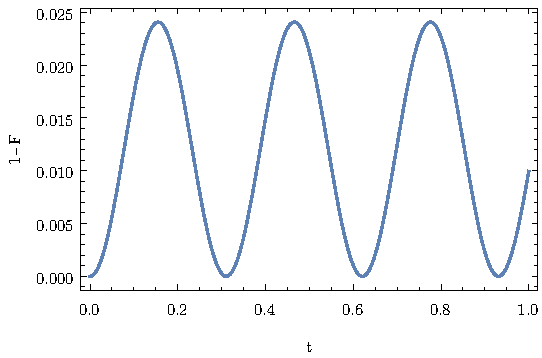
\includegraphics[scale=1.2]{../img/infidelityTimePlot.pdf}
    \caption{Fidelity in time for $T_f=10$}
    \label{fig:infidelityTimePlot}
\end{figure}
The \emph{final fidelity} (at $t=T_f$) dependence on final time $T_f$ can be seen on Fig. \ref{fig:infidelityTfPlot} and \ref{fig:infidelityTfPlotLog}.
\begin{figure}[H]
    \centering
    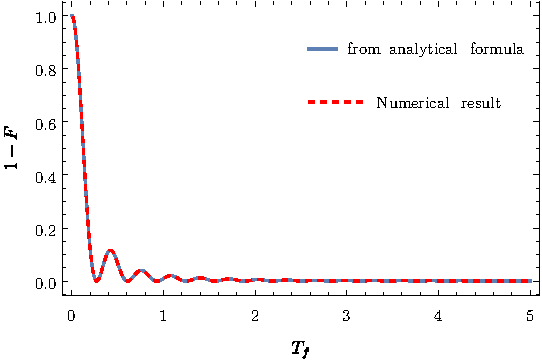
\includegraphics[scale=1.2]{../img/infidelityTfPlot.pdf}
    \caption{Final fidelity dependence on final time $T_f$.}
    \label{fig:infidelityTfPlot}
\end{figure}

\begin{figure}[H]
    \centering
    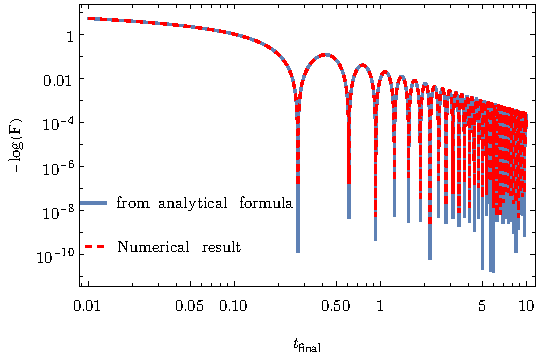
\includegraphics[scale=1.2]{../img/infidelityTfPlotLog.pdf}
    \caption{Fidelity dependence on final time in log-log scale. Spikes should go to zero, which does not hold due to numerical precision of the plotting algorithm.}
    \label{fig:infidelityTfPlotLog}
\end{figure}



From formula for fidelity \ref{eq:fidelitySimplified} goes $F=0$ is equivalent to
\begin{equation}
    a
\end{equation}

This proves that showing infidelity dependence on final time in log-log scale has spikes going to $0$, see Fig. \ref{fig:infidelityTfPlotLog}.



Fidelity as a function of time and final time can be seen on Figures \ref{fig:dens1}, \ref{fig:dens3}.
\begin{figure}[H]
    \centering
    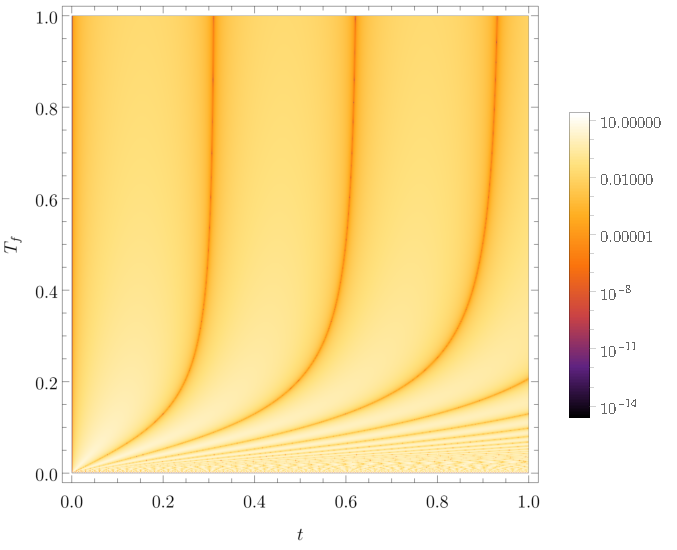
\includegraphics[scale=1.2]{../img/dens1.pdf}
    \caption{Fidelity dependence on time and final time.}
    \label{fig:dens1}
\end{figure}
\begin{figure}[H]
    \centering
    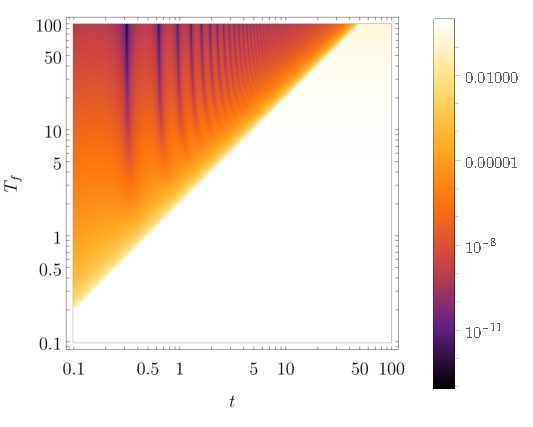
\includegraphics[scale=1.2]{../img/dens3.pdf}
    \caption{Fidelity dependence on time and final time in log log scale.}
    \label{fig:dens3}
\end{figure}

\section{Linear driving}

\begin{figure}[H]
    \centering
    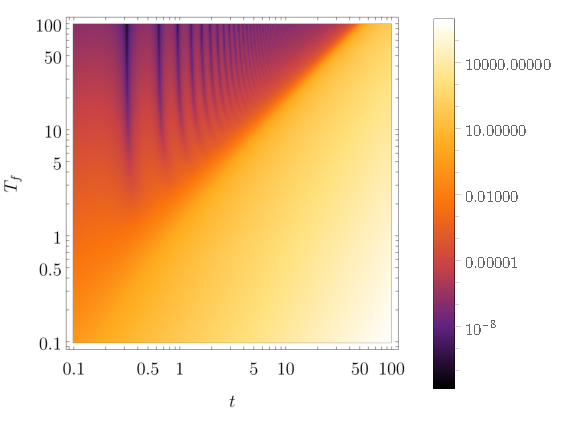
\includegraphics[scale=1.2]{../img/densVariance.pdf}
    \caption{Energy variance for $(\Lambda;\Omega)=(0;0.2)$ during the linear driving.}
    \label{fig:dens3}
\end{figure}